
\vspace{-10mm}
Amidakuji is a custom in Japan which 
allows for a pseudo-random assignment of children to prizes~\cite{A1}. 
Usually done in Japanese schools, a teacher will draw $n$ vertical lines, 
hereby known as \emph{lines}, where $n$ is the number of students in class. 
At the bottom of each line will be a unique prize. At the top of each line will be the name of one of the students.  
The teacher will then draw 0 or more horizontal lines, hereby known as \emph{bars}, 
connecting two adjacent lines. The more bars there are the more complicated (and fun) 
the Amidakuji is. No two endpoints of two bars can be touching. Each student then traces 
their line, and whenever they encounter an end point of a bar along their line, 
they must cross the bar and continue going down the adjacent line. 
The student continues tracing down the lines and crossing bars 
until they get to the end of the ladder lottery. We call such a tracing for a given student 
a \emph{path}. For example, the path of Ryu is highlighted in red in Figure~\ref{fig:aa}. The prize at the bottom of the ladder lottery 
is their prize~\cite{A1}. See Figure~\ref{fig:aa} for an example of a ladder lottery.
\begin{center}
\vspace{-5mm}
\begin{figure}[h]
	\centering
		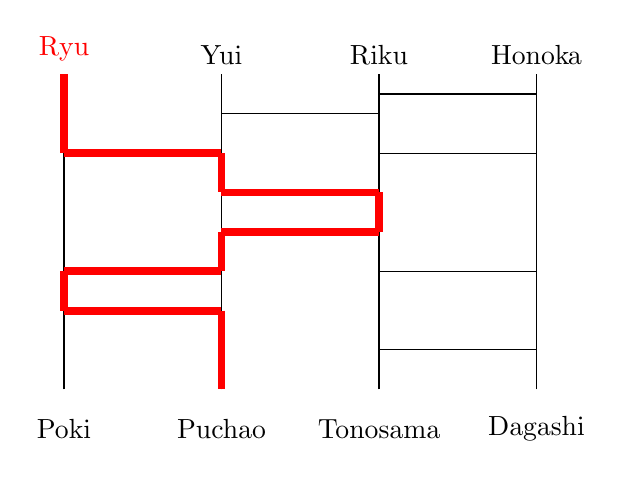
\begin{tikzpicture}
		%%Start of figure. Fig 1
			\draw(0, 0) to (0, 3); 
		
			\node at (0, -0.5){Poki};
			\draw(2, 0) to (2, 4) node[above]{Yui};
			\node at (2, -0.5){Puchao};
			\draw(4, 0) to (4, 4)node[above]{Riku};
			\node at (4, -0.5){Tonosama};
			\draw(6, 0) to (6, 4)node[above]{Honoka};
			\node at (6, -0.5){Dagashi};
			
			%bars%
		    \draw[line width=1mm, red](0, 3) to (0, 4) node[above]{Ryu};
			\draw[line width=1mm, red](0, 1) to (2, 1);
			\draw[line width=1mm, red](2, 1.5) to (2, 2);
			\draw[line width=1mm, red](0, 1)to(0, 1.5);
			\draw[line width=1mm, red](2, 1) to (2, 0);
			\draw[line width=1mm, red](0, 3) to (2, 3);
			\draw[line width=1mm, red](2, 3) to (2, 2.5);
			\draw[line width=1mm, red](4, 2) to (4, 2.5);
			\draw[line width=1mm, red](0, 1.5) to (2, 1.5);
			
			\draw[line width=1mm, red](2, 2) to (4, 2);
			\draw[line width=1mm, red](2, 2.5) to (4, 2.5);
			\draw(2, 3.5) to (4, 3.5);
			
			\draw(4, 0.5) to (6, 0.5);
			\draw(4, 3) to (6, 3);
			\draw(4, 1.5) to (6, 1.5);
			\draw(4, 3.75) to (6, 3.75);
		\end{tikzpicture}
\caption{A ladder lottery where Ryu gets Puchao, Yui gets Dagashi, Riku gets Tonosama and Honoka gets Poki}
\label{fig:aa}
\end{figure}
\end{center}
The game of Amidakuji has an interesting history. Amida is the Japanese name 
for Amithaba, the supreme Buddha of the Western Paradise. Amithaba
was a Buddha from India and there was a cult based around him. The cult 
of Amida, otherwise known as Amidism, believed that by worshiping Amithaba, they would 
enter into his Western Paradie. Amidism began in India in the fourth century,
made its way to China and Korea in the fifth century, and finally came 
to Japan in ninth century~\cite{A0}. Amidakuji began in Japan during 
the Muromachi period, which spanned from
1336 to 1573~\cite{A0}. During the Muromachi period, the game was played by having
players draw their names at the top of the lines, and at the bottom 
of the lines were pieces of paper that had the amount the players
were willing to bet. The pieces of paper were folded in the shape of 
Amithaba's halo. Kuji is the Japanese word for lottery. Hence, the game 
was termed Amidakuji. In English, Amidakuji translates to ladder lottery. 

An interesting property about a ladder lottery is that it is  
associated with a \emph{permutation}. A \emph{permutation} is a unique ordering of objects. 
For the purposes of this thesis, the objects of a permutation are $1,2, \dots ,n$. 
Consider a permutation $\pi=(p_{1},p_{2}, \dots ,p_{n})$.
A pair of elements, $p_{i}$ and $p_{j}$, form an \emph{inversion} if $p_{i}>p_{j}$ and $i<j$. 
For example, given $\pi=(4,3,5,1,2)$, its set of inversions is \newline $Inv=\{(4,3),(4,2),(4,1),(3,2),(3,1),(5,1),(5,2)\}$.
A \emph{transposition} is a swap of two elements in $\pi$.
An \emph{adjacent transposition} is defined as a swap of two adjacent elements in $\pi$.
Given $\pi_{1}=(4,3,5,1,2)$ and $\pi_{2}=(3,4,5,1,2)$, they differ by the adjacent 
transposition of the elements $(4,3)$.
A ladder lottery corresponds to a permutation when:
\begin{enumerate}
	\item The $n$ elements of $\pi$ are listed at the top of the ladder lottery in the order that they appear in 
	$\pi$; one element per line of the ladder lottery.
	\item At the bottom of the ladder lottery are the $n$ elements of $\pi$ in strictly ascending order. For 
	each element $x$ in $\pi$, $x$ goes down its path and ends up in the bottom $xth$ line. 
\end{enumerate} 

\subsection{Representation}
In this thesis, ladder lotteries are represented as a two dimensional array.
Let $n$ be the number of elements in $\pi$. Let a \emph{column} be a gap 
between lines in the ladder lottery. Each ladder lottery 
represented as a two dimensional array has $n-1$ columns. Let a \emph{row} 
be defined as a the horizontal span from column $1$ to column $n-1$ containing at least one bar. 
Let a \emph{ghost row} be defined as the horizontal span from column $1$ to column $n-1$ containing zero bars.
Let the \emph{height} of the ladder be defined as the number of 
rows plus the number of ghost rows in the ladder.
If two ladders are equivalent, then they sort $\pi$ with 
the exact same bars. If two ladders are identical, 
then they sort $\pi$ with the same exact same bars and with the same number of rows. 
In Figure~\ref{Fig:equivLadders}, all three ladders are equivalent but only the leftmost ladder 
and middle ladder are identical with two rows. The rightmost ladder 
has three rows. 
\begin{figure}[h]
	\centering
	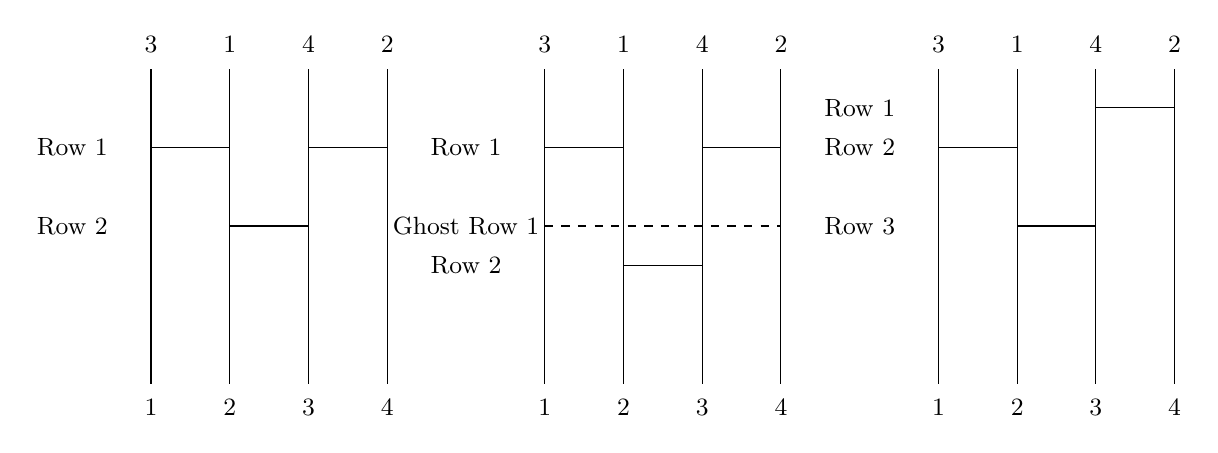
\begin{tikzpicture}
		\draw(0, 0) to (0, 4);
			\draw(0, 3) to (1, 3);
		\draw(1, 0) to (1, 4);
			\draw(1, 2) to (2, 2);
		\draw(2, 0) to (2, 4);
			\draw(2, 3) to (3, 3);
		\draw(3, 0) to (3, 4);
		
		\draw(5, 0) to (5, 4);
			\draw(5, 3) to (6, 3);
		\draw(6, 0) to (6, 4);
			\draw[dashed](5, 2)--(8, 2);
			\draw(6, 1.5) to (7, 1.5);
		\draw(7, 0) to (7, 4);
			\draw(7, 3) to (8, 3);
		\draw(8, 0) to (8, 4);


		\draw(10, 0) to (10, 4);
			\draw(10, 3) to (11, 3);
		\draw(11, 0) to (11, 4);
			\draw(11, 2) to (12, 2);
		\draw(12, 0) to (12, 4);
			\draw(12, 3.5) to (13, 3.5);
		\draw(13, 0) to (13, 4);


		\node at(0, 4.3){\small{$3$}};
		\node at(1, 4.3){\small{$1$}};
		\node at(2, 4.3){\small{$4$}};
		\node at(3, 4.3){\small{$2$}};
		
		\node at(5, 4.3){\small{$3$}};
		\node at(6, 4.3){\small{$1$}};
		\node at(7, 4.3){\small{$4$}};
		\node at(8, 4.3){\small{$2$}};
		
		\node at(10, 4.3){\small{$3$}};
		\node at(11, 4.3){\small{$1$}};
		\node at(12, 4.3){\small{$4$}};
		\node at(13, 4.3){\small{$2$}};

		\node at(0, -.3){\small{$1$}};
		\node at(1, -.3){\small{$2$}};
		\node at(2, -.3){\small{$3$}};
		\node at(3, -.3){\small{$4$}};
		
		\node at(5, -.3){\small{$1$}};
		\node at(6, -.3){\small{$2$}};
		\node at(7, -.3){\small{$3$}};
		\node at(8, -.3){\small{$4$}};
		
		\node at(10, -.3){\small{$1$}};
		\node at(11, -.3){\small{$2$}};
		\node at(12, -.3){\small{$3$}};
		\node at(13, -.3){\small{$4$}};

		\node at(-1, 3){\small{Row $1$}};
		\node at(-1, 2){\small{Row $2$}};


		\node at(4, 3){\small{Row $1$}};
		\node at(4, 2){\small{Ghost Row $1$}};
		\node at(4, 1.5){\small{Row $2$}};


		\node at(9, 3.5){\small{Row $1$}};
		\node at(9, 3){\small{Row $2$}};
		\node at(9, 2){\small{Row $3$}};
	\end{tikzpicture}
	\caption{Three equivalent ladders. Leftmost and middle ladders are identical.}
	\label{Fig:equivLadders}
\end{figure}


\subsection{Optimal Ladder Lotteries}
Let $k$ denote the number of inversions for some permutation.
An \emph{optimal ladder lottery} is a special case of ladder 
lottery, corresponding to $\pi$, in which there are $k$ bars in the ladder; one for each \emph{inversion} in $\pi$ such that each 
bar uninverts a single inversion in $\pi$ exactly once~\cite{A1}.
An optimal ladder lottery sorts $\pi$ in ascending order using exactly $k$ bars by applying 
$k$ adjacent transpositions on $k$ inversions in $\pi$.
For example, given $\pi=(4,3,5,1,2)$ an optimal ladder lottery associated with $\pi$ would have 
seven bars; one for each inversion in $\pi$. For each bar, two elements in $\pi$ that form 
an inversion cross the given bar. 
Once all elements have crossed their respective bars, $\pi$ is sorted in ascending order. The number of bars in an optimal ladder lottery 
is the lower bound for the number of bars in a ladder lottery required to sort $\pi$. 
To see an example of two ladder lotteries associated with 
$\pi=(4,3,5,1,2)$, one optimal and one non-optimal, please refer to Figure~\ref{fig:ab}.
\begin{figure}[h]
	\begin{minipage}{0.4\textwidth}
		\centering
		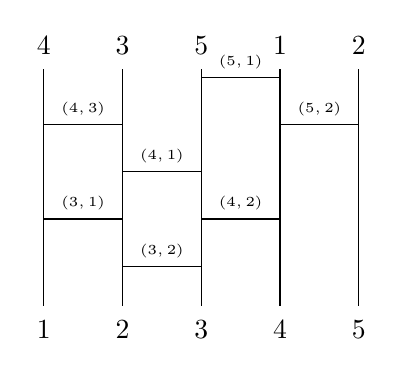
\begin{tikzpicture}
		 	\draw(0, 0) to (0, 3);
		 		\draw(0, 2.3) to (1, 2.3);
		 		\draw(0, 1.1) to (1, 1.1);

		 	\draw(1, 0) to (1, 3);
				 \draw(1, 1.7) to (2, 1.7);
				 \draw(1, .5) to (2, .5);
		 	\draw(2, 0) to (2, 3);
				 \draw(2, 2.9) to (3, 2.9);
				 \draw(2, 1.1) to (3, 1.1);
			 \draw(3, 0) to (3, 3);
			 	\draw(3, 2.3) to (4, 2.3);
			 \draw(4,0) to (4, 3);

			 \node at(0, 3.3){$4$};
			 \node at(1, 3.3){$3$};
			 \node at(2, 3.3){$5$};
			 \node at(3, 3.3){$1$};
			 \node at(4, 3.3){$2$};
			 \node at(0, -.3){$1$};
			 \node at(1, -.3){$2$};
			 \node at(2, -.3){$3$};
			 \node at(3, -.3){$4$};
			 \node at(4, -.3){$5$};

			 \node at(.5, 2.5){\tiny{$(4,3)$}};
			 \node at(.5, 1.3){\tiny{$(3,1)$}};
			 \node at(1.5, 1.9){\tiny{$(4,1)$}};
			 \node at(1.5, .7){\tiny{$(3,2)$}};
			 \node at(2.5, 3.1){\tiny{$(5,1)$}};
			 \node at(2.5, 1.3){\tiny{$(4,2)$}};
			 \node at(3.5, 2.5){\tiny{$(5,2)$}};


		\end{tikzpicture}
				

	\end{minipage}
	\begin{minipage}{.4\textwidth}
		\begin{flushright}
		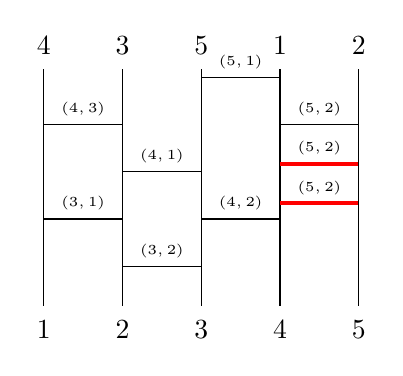
\begin{tikzpicture}
		 	\draw(0, 0) to (0, 3);
		 		\draw(0, 2.3) to (1, 2.3);
		 		\draw(0, 1.1) to (1, 1.1);

		 	\draw(1, 0) to (1, 3);
				 \draw(1, 1.7) to (2, 1.7);
				 \draw(1, .5) to (2, .5);
		 	\draw(2, 0) to (2, 3);
				 \draw(2, 2.9) to (3, 2.9);
				 \draw(2, 1.1) to (3, 1.1);
			 \draw(3, 0) to (3, 3);
				 \draw(3, 2.3) to (4, 2.3);
				 \draw [line width=0.5mm, red ](3, 1.8) to (4, 1.8);
				 \draw[line width=0.5mm, red ](3, 1.3) to (4, 1.3);
			 \draw(4,0) to (4, 3);

			 \node at(0, 3.3){$4$};
			 \node at(1, 3.3){$3$};
			 \node at(2, 3.3){$5$};
			 \node at(3, 3.3){$1$};
			 \node at(4, 3.3){$2$};
			 \node at(0, -.3){$1$};
			 \node at(1, -.3){$2$};
			 \node at(2, -.3){$3$};
			 \node at(3, -.3){$4$};
			 \node at(4, -.3){$5$};


			 \node at(.5, 2.5){\tiny{$(4,3)$}};
			 \node at(.5, 1.3){\tiny{$(3,1)$}};
			 \node at(1.5, 1.9){\tiny{$(4,1)$}};
			 \node at(1.5, .7){\tiny{$(3,2)$}};
			 \node at(2.5, 3.1){\tiny{$(5,1)$}};
			 \node at(2.5, 1.3){\tiny{$(4,2)$}};
			 \node at(3.5, 2.5){\tiny{$(5,2)$}};
			 \node at(3.5, 2.0){\tiny{$(5,2)$}};
			 \node at(3.5, 1.5){\tiny{$(5,2)$}};



		\end{tikzpicture}
	\end{flushright}
	\end{minipage}
	\caption{Two ladders for the permutation $(4,3,5,1,2)$. The left ladder is an optimal ladder and the right ladder is not. 
	The bold  bars in the right ladder are redundant, thus the right ladder is non optimal.}
	\label{fig:ab}
\end{figure}
Let $OptL\{\pi\}$ be defined as the set of optimal ladder lotteries that form an equivalence class, 
insofar as all ladders in $OptL\{\pi\}$ sort $\pi$ in ascending order with the least number of bars. The first discussion of 
$OptL\{\pi\}$ is in the paper Efficient Enumeration of Ladder Lotteries and its Application~\cite{A1}.
In this paper, the authors provide an algorithm known as {\sc FindAllChildren}
which generates $OptL\{\pi\}$; the details of the algorithm are discussed in Chapter 2.
To see $OptL\{(4,3,5,1,2)\}$ please refer to Figure \ref{Fig:OptL3421}.
Given that there are $n!$ permutations of order $n$, each of them 
have their own $OptL\{\pi\}$. In Table~\ref{table:KInvOptL} found in the appendix, 
the number of ladders in each of the 120 $OptL\{\pi\}$ of order $5$ is presented.\pagebreak
\begin{figure}[t]
	\centering
	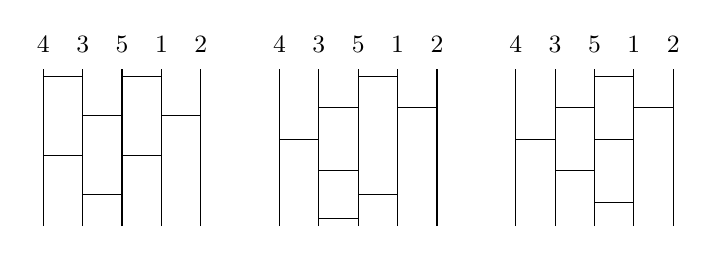
\begin{tikzpicture}
		\draw(0,0) to (0,2);
			\draw(0, 1.9) to (.5, 1.9);
			\draw(0, .9) to (.5, .9);
		\draw(.5,0) to (0.5,2);
			\draw(.5, 1.4) to (1, 1.4);
			\draw(.5, .4) to (1, .4);
		\draw(1,0) to (1,2);
			\draw(1, 1.9) to (1.5, 1.9);
			\draw(1, .9) to (1.5, .9);
		\draw(1.5,0) to (1.5,2);
			\draw(1.5, 1.4) to (2, 1.4);
		\draw(2,0) to (2,2);

		\draw(3, 0) to (3, 2);
			\draw(4, 1.9) to (4.5, 1.9);
			\draw(3.5, 1.5) to (4, 1.5);
			\draw(4.5, 1.5) to (5, 1.5);
			\draw(3.5, 1.1) to (3, 1.1);
			\draw(3.5, 0.7) to (4, 0.7);
			\draw(4, .4) to (4.5, .4);
			\draw(3.5, .1) to (4, .1);
		\draw(3.5, 0) to (3.5, 2);
		\draw(4, 0) to (4, 2);
		\draw(4.5, 0) to (4.5, 2);
		\draw(5, 0) to (5, 2);

		\draw(6, 0) to (6, 2);
			\draw(7.5, 1.9) to (7, 1.9);
			\draw(6.5, 1.5) to (7, 1.5);
			\draw(7.5, 1.5) to (8, 1.5);
			\draw(6, 1.1) to (6.5, 1.1);
			\draw(7, 1.1) to (7.5, 1.1);
			\draw(6.5, 0.7) to (7, 0.7);
			\draw(7, 0.3) to (7.5, 0.3);
		\draw(6.5, 0) to (6.5, 2);
		\draw(7, 0) to (7, 2);
		\draw(7.5, 0) to (7.5, 2);
		\draw(8, 0) to (8, 2);

		\node at(0, 2.3){\small{$4$}};
		\node at(.5, 2.3){\small{$3$}};
		\node at(1, 2.3){\small{$5$}};
		\node at(1.5, 2.3){\small{$1$}};
		\node at(2, 2.3){\small{$2$}};

		\node at(3, 2.3){\small{$4$}};
		\node at(3.5, 2.3){\small{$3$}};
		\node at(4, 2.3){\small{$5$}};
		\node at(4.5, 2.3){\small{$1$}};
		\node at(5, 2.3){\small{$2$}};

		\node at(6, 2.3){\small{$4$}};
		\node at(6.5, 2.3){\small{$3$}};
		\node at(7, 2.3){\small{$5$}};
		\node at(7.5, 2.3){\small{$1$}};
		\node at(8, 2.3){\small{$2$}};
	\end{tikzpicture}
	\caption{All the optimal ladders in $OptL\{(4,3,5,1,2)\}$}
	\label{Fig:OptL3421}
\end{figure}

\subsection{Combinatorial Generation}
Our research on ladder lotteries pertains to research in \emph{combinatorial generation}. Combinatorial 
generation is a subfield of theoretical computer science which lists all instances of  
combinatorial objects such as permutations, combinations, sets, subsets, graphs, and ladder lotteries. Gray codes are a 
special type of combinatorial generation in which a constant amount of constant change 
is required to get from one object to the next. For example, a single swap operation,
a single rotation, or a single bit flip is used to get from one object to the next. The term
``Gray Code" comes from the Binary Reflected code for binary strings given by Frank Gray~\cite{A39}.
There are many known algorithms for listing permutations of order $n$. Throughout the course of this thesis,
a number of such algorithms were researched~\cite{A18,A19,A21,A24,A25,A26,A31,A34,A35,A36,A37}.
Each of these algorithms will be reviewed in Chapter 2. 
To see all $24$ ladders listed in lexicographic order please refer to Figure~\ref{Fig:TwentyFour}.
\begin{figure}[!htp]
	\centering
	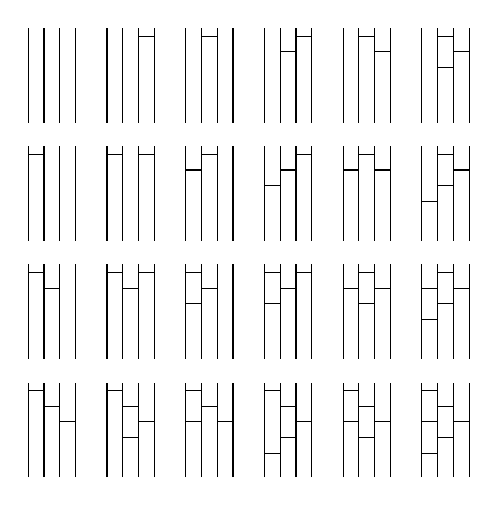
\begin{tikzpicture}
	\draw(0.00,5.90) to (0.00,7.10);
	\draw(0.20,5.90) to (0.20,7.10);
	\draw(0.40,5.90) to (0.40,7.10);
	\draw(0.60,5.90) to (0.60,7.10);
	\draw(1.00,5.90) to (1.00,7.10);
	\draw(1.20,5.90) to (1.20,7.10);
	\draw(1.40,5.90) to (1.40,7.10);
	\draw(1.60,5.90) to (1.60,7.10);
	\draw(1.40, 7.00) to (1.60, 7.00);
	\draw(2.00,5.90) to (2.00,7.10);
	\draw(2.20,5.90) to (2.20,7.10);
	\draw(2.40,5.90) to (2.40,7.10);
	\draw(2.60,5.90) to (2.60,7.10);
	\draw(2.20, 7.00) to (2.40, 7.00);
	\draw(3.00,5.90) to (3.00,7.10);
	\draw(3.20,5.90) to (3.20,7.10);
	\draw(3.40,5.90) to (3.40,7.10);
	\draw(3.60,5.90) to (3.60,7.10);
	\draw(3.40, 7.00) to (3.60, 7.00);
	\draw(3.20, 6.80) to (3.40, 6.80);
	\draw(4.00,5.90) to (4.00,7.10);
	\draw(4.20,5.90) to (4.20,7.10);
	\draw(4.40,5.90) to (4.40,7.10);
	\draw(4.60,5.90) to (4.60,7.10);
	\draw(4.20, 7.00) to (4.40, 7.00);
	\draw(4.40, 6.80) to (4.60, 6.80);
	\draw(5.00,5.90) to (5.00,7.10);
	\draw(5.20,5.90) to (5.20,7.10);
	\draw(5.40,5.90) to (5.40,7.10);
	\draw(5.60,5.90) to (5.60,7.10);
	\draw(5.20, 7.00) to (5.40, 7.00);
	\draw(5.40, 6.80) to (5.60, 6.80);
	\draw(5.20, 6.60) to (5.40, 6.60);
	
	\draw(0.00,4.40) to (0.00,5.60);
	\draw(0.20,4.40) to (0.20,5.60);
	\draw(0.40,4.40) to (0.40,5.60);
	\draw(0.60,4.40) to (0.60,5.60);
	\draw(0.00, 5.50) to (0.20, 5.50);
	\draw(1.00,4.40) to (1.00,5.60);
	\draw(1.20,4.40) to (1.20,5.60);
	\draw(1.40,4.40) to (1.40,5.60);
	\draw(1.60,4.40) to (1.60,5.60);
	\draw(1.00, 5.50) to (1.20, 5.50);
	\draw(1.40, 5.50) to (1.60, 5.50);
	\draw(2.00,4.40) to (2.00,5.60);
	\draw(2.20,4.40) to (2.20,5.60);
	\draw(2.40,4.40) to (2.40,5.60);
	\draw(2.60,4.40) to (2.60,5.60);
	\draw(2.20, 5.50) to (2.40, 5.50);
	\draw(2.00, 5.30) to (2.20, 5.30);
	\draw(3.00,4.40) to (3.00,5.60);
	\draw(3.20,4.40) to (3.20,5.60);
	\draw(3.40,4.40) to (3.40,5.60);
	\draw(3.60,4.40) to (3.60,5.60);
	\draw(3.40, 5.50) to (3.60, 5.50);
	\draw(3.20, 5.30) to (3.40, 5.30);
	\draw(3.00, 5.10) to (3.20, 5.10);
	\draw(4.00,4.40) to (4.00,5.60);
	\draw(4.20,4.40) to (4.20,5.60);
	\draw(4.40,4.40) to (4.40,5.60);
	\draw(4.60,4.40) to (4.60,5.60);
	\draw(4.20, 5.50) to (4.40, 5.50);
	\draw(4.00, 5.30) to (4.20, 5.30);
	\draw(4.40, 5.30) to (4.60, 5.30);
	\draw(5.00,4.40) to (5.00,5.60);
	\draw(5.20,4.40) to (5.20,5.60);
	\draw(5.40,4.40) to (5.40,5.60);
	\draw(5.60,4.40) to (5.60,5.60);
	\draw(5.20, 5.50) to (5.40, 5.50);
	\draw(5.40, 5.30) to (5.60, 5.30);
	\draw(5.20, 5.10) to (5.40, 5.10);
	\draw(5.00, 4.90) to (5.20, 4.90);
	
	\draw(0.00,2.90) to (0.00,4.10);
	\draw(0.20,2.90) to (0.20,4.10);
	\draw(0.40,2.90) to (0.40,4.10);
	\draw(0.60,2.90) to (0.60,4.10);
	\draw(0.00, 4.00) to (0.20, 4.00);
	\draw(0.20, 3.80) to (0.40, 3.80);
	\draw(1.00,2.90) to (1.00,4.10);
	\draw(1.20,2.90) to (1.20,4.10);
	\draw(1.40,2.90) to (1.40,4.10);
	\draw(1.60,2.90) to (1.60,4.10);
	\draw(1.00, 4.00) to (1.20, 4.00);
	\draw(1.40, 4.00) to (1.60, 4.00);
	\draw(1.20, 3.80) to (1.40, 3.80);
	\draw(2.00,2.90) to (2.00,4.10);
	\draw(2.20,2.90) to (2.20,4.10);
	\draw(2.40,2.90) to (2.40,4.10);
	\draw(2.60,2.90) to (2.60,4.10);
	\draw(2.00, 4.00) to (2.20, 4.00);
	\draw(2.20, 3.80) to (2.40, 3.80);
	\draw(2.00, 3.60) to (2.20, 3.60);
	\draw(3.00,2.90) to (3.00,4.10);
	\draw(3.20,2.90) to (3.20,4.10);
	\draw(3.40,2.90) to (3.40,4.10);
	\draw(3.60,2.90) to (3.60,4.10);
	\draw(3.00, 4.00) to (3.20, 4.00);
	\draw(3.40, 4.00) to (3.60, 4.00);
	\draw(3.20, 3.80) to (3.40, 3.80);
	\draw(3.00, 3.60) to (3.20, 3.60);
	\draw(4.00,2.90) to (4.00,4.10);
	\draw(4.20,2.90) to (4.20,4.10);
	\draw(4.40,2.90) to (4.40,4.10);
	\draw(4.60,2.90) to (4.60,4.10);
	\draw(4.20, 4.00) to (4.40, 4.00);
	\draw(4.00, 3.80) to (4.20, 3.80);
	\draw(4.40, 3.80) to (4.60, 3.80);
	\draw(4.20, 3.60) to (4.40, 3.60);
	\draw(5.00,2.90) to (5.00,4.10);
	\draw(5.20,2.90) to (5.20,4.10);
	\draw(5.40,2.90) to (5.40,4.10);
	\draw(5.60,2.90) to (5.60,4.10);
	\draw(5.20, 4.00) to (5.40, 4.00);
	\draw(5.00, 3.80) to (5.20, 3.80);
	\draw(5.40, 3.80) to (5.60, 3.80);
	\draw(5.20, 3.60) to (5.40, 3.60);
	\draw(5.00, 3.40) to (5.20, 3.40);
	
	\draw(0.00,1.40) to (0.00,2.60);
	\draw(0.20,1.40) to (0.20,2.60);
	\draw(0.40,1.40) to (0.40,2.60);
	\draw(0.60,1.40) to (0.60,2.60);
	\draw(0.00, 2.50) to (0.20, 2.50);
	\draw(0.20, 2.30) to (0.40, 2.30);
	\draw(0.40, 2.10) to (0.60, 2.10);
	\draw(1.00,1.40) to (1.00,2.60);
	\draw(1.20,1.40) to (1.20,2.60);
	\draw(1.40,1.40) to (1.40,2.60);
	\draw(1.60,1.40) to (1.60,2.60);
	\draw(1.00, 2.50) to (1.20, 2.50);
	\draw(1.20, 2.30) to (1.40, 2.30);
	\draw(1.40, 2.10) to (1.60, 2.10);
	\draw(1.20, 1.90) to (1.40, 1.90);
	\draw(2.00,1.40) to (2.00,2.60);
	\draw(2.20,1.40) to (2.20,2.60);
	\draw(2.40,1.40) to (2.40,2.60);
	\draw(2.60,1.40) to (2.60,2.60);
	\draw(2.00, 2.50) to (2.20, 2.50);
	\draw(2.20, 2.30) to (2.40, 2.30);
	\draw(2.00, 2.10) to (2.20, 2.10);
	\draw(2.40, 2.10) to (2.60, 2.10);
	\draw(3.00,1.40) to (3.00,2.60);
	\draw(3.20,1.40) to (3.20,2.60);
	\draw(3.40,1.40) to (3.40,2.60);
	\draw(3.60,1.40) to (3.60,2.60);
	\draw(3.00, 2.50) to (3.20, 2.50);
	\draw(3.20, 2.30) to (3.40, 2.30);
	\draw(3.40, 2.10) to (3.60, 2.10);
	\draw(3.20, 1.90) to (3.40, 1.90);
	\draw(3.00, 1.70) to (3.20, 1.70);
	\draw(4.00,1.40) to (4.00,2.60);
	\draw(4.20,1.40) to (4.20,2.60);
	\draw(4.40,1.40) to (4.40,2.60);
	\draw(4.60,1.40) to (4.60,2.60);
	\draw(4.00, 2.50) to (4.20, 2.50);
	\draw(4.20, 2.30) to (4.40, 2.30);
	\draw(4.00, 2.10) to (4.20, 2.10);
	\draw(4.40, 2.10) to (4.60, 2.10);
	\draw(4.20, 1.90) to (4.40, 1.90);
	\draw(5.00,1.40) to (5.00,2.60);
	\draw(5.20,1.40) to (5.20,2.60);
	\draw(5.40,1.40) to (5.40,2.60);
	\draw(5.60,1.40) to (5.60,2.60);
	\draw(5.00, 2.50) to (5.20, 2.50);
	\draw(5.20, 2.30) to (5.40, 2.30);
	\draw(5.00, 2.10) to (5.20, 2.10);
	\draw(5.40, 2.10) to (5.60, 2.10);
	\draw(5.20, 1.90) to (5.40, 1.90);
	\draw(5.00, 1.70) to (5.20, 1.70);
	
	\end{tikzpicture}
	\caption{All $24$ ladders listed in lexicographic order.}
	\label{Fig:TwentyFour}
\end{figure}


\section{Thesis Statement}
  	This thesis considers a combinatorial generation problem related 
    to ladder lotteries. The problem is the so called Canonical Ladder Listing Problem. 
	This problem asks, given all $n!$ permutations of order $n$, is there an efficient algorithm for listing 
	one optimal ladder per permutation? In other words, 
	is there an easy way to transition from one ladder to the next until all $n!$ ladders 
	have been listed? In this thesis, 'N' of the aforementioned permutation listing algorithms are modified in order to 
	list $n!$ ladder lotteries, each of which corresponds to one of the $n!$ permutations of order $n$. 
	The first of these algorithms is a modification of the Steinhaus-Johnson-Trotter algorithm; SJT for short~\cite{A25}. 
	
	%%%Write a second part on ER if he decides you need it.

	

	

\section{Contributions}
	For the Canonical Ladder Listing Problem, this thesis provides 
	a number of algorithms for listing all $n!$ ladders. These algorithms are termed Algorithm~\ref{Alg:RootLadder} which 
	can be found in Chapter 3, {\sc ModifiedSJT} which 
	can be found in Chapter 3, Algorithm~\ref{Alg:ModSJT}, and {\sc CyclicBar} which can be found in Chapter 3 Algorithm~\ref{Alg:KInv}.
	This thesis also provides a number of theorems and lemmas relating to The Canonical Ladder Listing Problem. Furthermore, we define the 
	\emph{canonical representation of the root ladder} which can be found in Chapter 3.
	

\section{Summary of Past Known Results}
To the best of my knowledge, the first paper written on ladder lotteries is titled Efficient Enumeration of 
Ladder Lotteries and its Application written by Yamanaka, Nakano, Matsui Uehara and Nakada. The paper 
was written in 2010~\cite{A1}. Since this paper, 
a number of problems related to ladder lotteries have been solved. In Table~\ref{Table:KnownProblems} 
the reader will find a table of solved problems related to ladder lotteries. In Chapter 2 a more comprehensive analysis of these 
solved problems will be provided.
\begin{table}[h]
	\centering
	\begin{tabular}{|p{4cm}||p{4cm}||p{4cm}|}
		\hline 
		\multicolumn{3}{|c|}{Table of Known Results Related to Ladder Lotteries}\\
		\hline 
		\hline 
		Name of Problem & Description & Source \\ 
		\hline 
		\small{Enumeration Problem} & \small{Generates $OptL\{\pi\}$} &~\cite{A1} 2010\\ 
		\hline
		\small{Ladder Lottery \newline Realization Problem} & \small{Determines time complexity for creating a ladder lottery given a multi-set of bars} &~\cite{A3} 2018\\ 
		\hline
		\small{The Reconfiguration \newline Problem} & \small{Determine the length of the path between two ladders in $OptL\{\pi\}$} &~\cite{A2} 2017\\ 
		\hline 
		\small{Enumeration Problem \newline given $n$, $k$} & \small{Generates all ladders with $n$ lines and $k$ bars; includes non-optimal ladders} &~\cite{A4} 2014\\ 
		\hline
		\small{The Coding Problem} & \small{Provides a binary string encoding for a ladder lottery} &~\cite{A5} 2012\\ 
		\hline 
		\small{Counting and \newline Random Generation \newline Problem} & \small{Provides a solution for counting ladder lotteries of a given type as well as randomly generating a ladder lottery} &~\cite{A6} 2017\\ 
		\hline
		
																



	\end{tabular}
	\caption{Table of known solutions for problems related to ladder lotteries}
	\label{Table:KnownProblems}
\end{table}

\section{Overview of Thesis}
This thesis is broken down into several sections. In Chapter 2, a literature
review of ladder lotteries will be provided along with background information pertinent to this thesis. 
In Chapter 3, The canonical configuration of the root ladder is provided. 
Chapter 3 is broken down into four subsections. The first subsection is the introduction to the problem, 
the second is a methodology subsection, the third is a results 
subsection and the fourth is a conclusion/analysis subsection. 
In Chapter 4, The {\sc ModifiedSJT} algorithm is provided. Chapter 4 is broken down into four subsections.
The first subsection is the introduction to the algorithm, 
the second is a methodology subsection, the third is a results 
subsection and the fourth is a conclusion/analysis subsection. In Chapter 5, The {\sc K-Bar Generation} algorithms 
are provided. The first subsection is the introduction to the algorithms, 
the second is a methodology subsection, the third is a results 
subsection and the fourth is a conclusion/analysis subsection. 